\begin{frame}{CONNExIN: building expertise, looking toward Lagos}
  \begin{columns}[c,onlytextwidth]
    \column{.67\textwidth}
      \small
  \NTXPoint{Udunna Anazodo and the CONNExIN team}{Hybrid, hands-on neuroimaging training: developing local experts who can train others.}
  \NTXPoint{A shared contribution at ISMRM 2026}{Draper et al., abstract 563-01-002.\newline Morgan Hough, NeuroTechX --- co-author.}
  {\scriptsize\itshape Training 105 African clinicians and students in open neuroimaging analysis: CAMERA's dementia research program\par}
  \medskip
  \NTXPoint{Our hope for Lagos}{To become the first NeuroTechX city chapter in sub-Saharan Africa --- an ambition we hope to realize.}
    \column{.28\textwidth}
      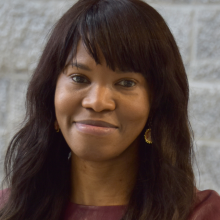
\includegraphics[width=\linewidth,height=35mm,keepaspectratio]{assets/people/udunna-anazodo.png}\par\smallskip
      {\small Udunna Anazodo\par}
      {\tiny Portrait: \href{https://mcmedhacks.com/team/dr-udunna-anazodo/}{McMedHacks}\par}
  \end{columns}
  {\tiny\color{NTXMuted}Sources: \href{https://event.fourwaves.com/connexin/pages/41f08c9e-6502-46b4-bf53-ec5a6cf095b7}{CONNExIN program}; \href{https://echo.ismrm.org/abstracts/view/a98f4909-2b73-49d0-849b-14f932d68bca}{ISMRM 2026 abstract}; Lagos aspiration: Morgan Hough\par}
  \note{[73:15--74:45] The official program spelling is CONNExIN. Credit Udunna Anazodo and the whole team. Its organizers describe a free hybrid train-the-trainer initiative connecting the MiND Lab at the Montreal Neurological Institute with McGill's aging research centre, the Medical Artificial Intelligence Lab in Nigeria, and CAMERA. Team-based learning builds local neuroimaging expertise. The 2025 program lists the MAI Lab in Lagos as its hybrid location. The accepted ISMRM 2026 digital-poster abstract is Training 105 African clinicians and students in open neuroimaging analysis: CAMERA's dementia research program, presented by Ethan Draper in Cape Town on May 13. Morgan is listed as a co-author with NeuroTechX affiliation. The title's 105 is not independently verified as a completion or certification count: the full abstract and results are access-restricted and were not read. Our hope is for Lagos to become the first NTX city chapter in sub-Saharan Africa. This is Morgan's aspiration, not a claim that a chapter has launched or an independently audited first-ever ranking. The public NTX directory mentions Lagos without proving launch status. Do not conflate this with the existing ISMRM African Chapter or imply that NTX owns CONNExIN.}
\end{frame}
